\documentclass[11pt]{article}
\usepackage[margin=2.5cm]{geometry}
\usepackage{amsmath,amssymb,amsthm}
\usepackage{graphicx}
\usepackage{booktabs}
\usepackage{hyperref}
\usepackage{xcolor}
\usepackage{listings}
\usepackage{microtype}
\usepackage{caption}
\usepackage{float}

\lstset{
  basicstyle=\ttfamily\small,
  showstringspaces=false,
  breaklines=true,
  frame=single,
  framesep=3pt,
  xleftmargin=6pt,
  xrightmargin=6pt,
}

\newtheorem{proposition}{Proposition}
\theoremstyle{definition}
\newtheorem{definition}{Definition}
\newtheorem{remark}{Remark}

\title{\textbf{Milestone M2: \texttt{TaylorSeries.jl}}\\[0.4em]
\large Certified Taylor-Series Bounds Between Grid Points\\[0.2em]
\normalsize \texttt{wave-cap} --- Computer-Assisted Proof for the Babenko Equation}
\author{BabenkoRigorous.jl}
\date{May 2026}

\begin{document}
\maketitle

\begin{abstract}
We describe the implementation and validation of \texttt{TaylorSeries.jl},
the certified Taylor-series layer of the \texttt{BabenkoRigorous.jl} package.
The module provides rigorous upper and lower bounds on smooth $2\pi$-periodic
functions between equispaced grid points using the Taylor remainder formula.
The struct carries, at each grid point, the per-derivative values
$f^{(m)}(u_j)$ for $m=0,\ldots,M_{\mathrm{order}}$ and, globally, a
\emph{vector} of certified supremum-norm bounds
$\texttt{sup\_bounds}[m+1] \ge \|f^{(m)}\|_\infty$ for $m=0,\ldots,M_{\mathrm{order}}+1$.
This vector representation (a port of the design used in \texttt{ccf-cap}'s
\texttt{CCFBlowup.jl}) is structurally what the Leibniz and Faà di Bruno
bounds require for products, inverses, and square roots; an earlier single-scalar
\texttt{F\_bound} representation was insufficient. All ten milestone tests pass
(393/393 assertions): the Taylor expansion contains the true function value
at 200 test points (T2.1); \texttt{sup\_bound} exceeds $\|\sin\|_\infty = 1$
(T2.2); a certified lower bound $D_{\mathrm{lower}} \approx 0.8999$ is
established for $y = 0.1\cos u$ (true $D_{\min} = 0.9$) (T2.3); the
overestimate decays rapidly with Taylor order (T2.4); \texttt{deriv\_series},
product, and \texttt{inv\_series} pass pointwise checks (T2.5--T2.7); and
new rigour tests (T2.8--T2.10) verify the \texttt{sup\_bounds} vectors of
products, \texttt{inv\_series}, and \texttt{sqrt\_series} respond correctly
to high-frequency input (audit C1--C4 regression coverage).
\end{abstract}

\tableofcontents
\bigskip

%% -------------------------------------------------------------------
\section{Background and motivation}

The Babenko water-wave residual (detailed in the M1 report)
involves the quantity
\[
  D(u) = \sqrt{y_u(u)^2 + (1 + \hat H[y_u](u))^2},
\]
which appears in the denominator of the curvature terms.
Bounding $\|R\|_{L^\infty([0,2\pi])}$ requires
\begin{itemize}
  \item a certified \emph{upper} bound on $\|R\|_\infty$, which needs an upper
        bound on $\|1/D\|_\infty$;
  \item a certified \emph{lower} bound $D_{\min} > 0$ on $D(u)$ over the whole
        interval (not just at grid points).
\end{itemize}

Milestone M1 provided \texttt{supnorm\_bound} for trig polynomials using the
$\ell^1$-norm bound on Fourier coefficients (see the M1 report).
However, the function $1/D$ is \emph{not} a trig polynomial, so a different
approach is required between grid points.

\textbf{The key idea of M3.}
For a smooth function $f$ on $[0,2\pi]$, if we know $f(u_j),\ldots,f^{(M)}(u_j)$
at each grid point $u_j$ and have a global bound $F$ on $|f^{(M+1)}|$, then
Taylor's theorem with remainder gives, for any $u \in [u_j, u_{j+1}]$:
\begin{equation}\label{eq:taylor}
  f(u) = \sum_{m=0}^{M} \frac{f^{(m)}(u_j)}{m!}(u - u_j)^m + R_j(u),
  \qquad |R_j(u)| \le \frac{F \cdot h^{M+1}}{(M+1)!},
\end{equation}
where $h = 2\pi / M_{\mathrm{grid}}$.
This gives certified pointwise bounds on $f$ over every subinterval, and hence
over all of $[0,2\pi]$.

%% -------------------------------------------------------------------
\section{Mathematical content}

\subsection{The \texttt{TaylorSeries} struct}

\begin{definition}
A \emph{\texttt{TaylorSeries}} for a smooth $2\pi$-periodic function $f$
consists of:
\begin{align*}
  &\texttt{derivs}[j, m+1] = f^{(m)}(u_j) \in \mathbb{R},
  \quad j = 1,\ldots,M_{\mathrm{grid}},\; m = 0,\ldots,M_{\mathrm{order}},\\
  &\texttt{sup\_bounds}[m+1] \ge \sup_{u \in [0,2\pi]} |f^{(m)}(u)|,
  \quad m = 0,\ldots,M_{\mathrm{order}}+1,
\end{align*}
where $u_j = 2\pi(j-1)/M_{\mathrm{grid}}$ and $h = 2\pi/M_{\mathrm{grid}}$.
All values are stored as \texttt{Arb} balls. The \texttt{sup\_bounds} vector
has length $M_{\mathrm{order}}+2$, indexed $1$ through $M_{\mathrm{order}}+2$.
\end{definition}

\begin{remark}
The Taylor remainder uses only \texttt{sup\_bounds[end]} (the top-derivative
bound), but the Leibniz formula for products and the Faà di Bruno formula
for $1/f$ and $\sqrt{f}$ require bounds on \emph{every} intermediate derivative.
The earlier single-scalar \texttt{F\_bound} representation could only express
the top derivative, leading to unsound formulas in $1/f$, $\sqrt{f}$, and the
product that ignored intermediate-derivative bounds entirely. Carrying the
full vector resolves this structurally.
\end{remark}

\subsection{Certified sup and inf bounds}

\begin{proposition}[Sup bound]\label{prop:sup}
Write $F = \texttt{sup\_bounds}[M{+}2]$ for the top-derivative supnorm bound.
For each $j = 1,\ldots,M_{\mathrm{grid}}$ and $u \in [u_j, u_j + h]$:
\[
  |f(u)| \le \sum_{m=0}^{M} \frac{|f^{(m)}(u_j)|}{m!} h^m
              + \frac{F \cdot h^{M+1}}{(M+1)!} =: S_j.
\]
Therefore $\|f\|_\infty \le \max_j S_j$.
\end{proposition}

\begin{proposition}[Inf bound]\label{prop:inf}
With $F$ as above, for each $j$ and $u \in [u_j, u_j + h]$:
\[
  f(u) \ge f(u_j) - \sum_{m=1}^{M} \frac{|f^{(m)}(u_j)|}{m!} h^m
           - \frac{F \cdot h^{M+1}}{(M+1)!} =: L_j.
\]
Therefore $\min_{u \in [0,2\pi]} f(u) \ge \min_j L_j$.
\end{proposition}

Both bounds follow directly from \eqref{eq:taylor} and the triangle inequality.
Only the top-derivative bound enters the remainder term; the other entries
of \texttt{sup\_bounds} are used by the arithmetic operations below.

\subsection{Arithmetic operations}

\paragraph{Differentiation (\texttt{deriv\_series}).}
The $m$-th derivative of $f'$ is the $(m+1)$-th derivative of $f$:
\[
  (f')^{(m)}(u_j) = f^{(m+1)}(u_j),
  \qquad
  \texttt{sup\_bounds}_{f'}[m+1] = \texttt{sup\_bounds}_{f}[m+2].
\]
The new \texttt{sup\_bounds} vector is just the old vector shifted left by
one entry (and is therefore of length $(M_{\mathrm{order}}{+}1){+}1 = M_{\mathrm{order}}{+}1$
for the new series of order $M_{\mathrm{order}}{-}1$). No spurious looseness factor
is introduced — the new top-derivative bound is exactly the old
$\texttt{sup\_bounds}[M{+}2]$.

\paragraph{Addition and scalar multiplication.}
These are pointwise. The new \texttt{sup\_bounds} vector is the entry-wise
triangle inequality $\texttt{sup\_bounds}_{f+g}[m+1] = \texttt{sup\_bounds}_f[m+1] + \texttt{sup\_bounds}_g[m+1]$
(respectively $|c| \cdot \texttt{sup\_bounds}_f[m+1]$).

\paragraph{Multiplication.}
The $m$-th derivative of $fg$ is the Leibniz rule:
\[
  (fg)^{(m)} = \sum_{k=0}^{m} \binom{m}{k} f^{(k)} g^{(m-k)}.
\]
Applying the triangle inequality term-by-term — and using the same Leibniz
formula \emph{at every order} $m = 0,\ldots,M_{\mathrm{order}}+1$ — gives
the \emph{exact-Leibniz} sup\_bounds vector:
\begin{equation}\label{eq:product_fbound}
  \texttt{sup\_bounds}_{fg}[m{+}1]
    = \sum_{k=0}^{m} \binom{m}{k}\, \texttt{sup\_bounds}_f[k{+}1]\,
                                    \texttt{sup\_bounds}_g[m{-}k{+}1].
\end{equation}
This is rigorous because binomial coefficients are non-negative and the
sup\_bounds vectors entries are themselves non-negative, so triangle inequality
applies term-by-term. The formula is the sharpest bound that uses only
per-derivative supnorms (no log-convexity / Landau--Kolmogorov interpolation
assumed). An earlier conservative formula
$F_{fg} = 2^{M+1}(F_f \cdot S_g + S_f \cdot F_g)$ used only the top-and-bottom
supnorms; it failed to bound the intermediate cross terms of Leibniz on
high-frequency inputs.\footnote{For $f = g = \cos(Nu)$ with sup-norm 1 and
$(M{+}1)$-th derivative norm $N^{M+1}$, the intermediate Leibniz term at
$k = (M{+}1)/2$ contributes $\binom{M+1}{(M+1)/2} \cdot N^{(M+1)/2} \cdot N^{(M+1)/2}
= \binom{M+1}{(M+1)/2} \cdot N^{M+1}$, which the old formula did not capture.}

\subsection{Recursive formulas for composed functions}

\subsubsection{Inverse (\texttt{inv\_series})}

Given $f \ge d_{\min} > 0$, the per-grid-point derivatives of $g = 1/f$
are computed by the standard recursion:
\begin{align}
  g^{(0)} &= 1/f^{(0)}, \label{eq:inv0}\\
  g^{(m)} &= -\frac{1}{f^{(0)}} \sum_{k=1}^{m} \binom{m}{k} f^{(k)} g^{(m-k)},
             \quad m \ge 1. \label{eq:invm}
\end{align}
This follows from differentiating $f \cdot g = 1$ and solving for $g^{(m)}$.

\textbf{\texttt{sup\_bounds} via Fa\`a di Bruno composition.}
The outer function $\phi(x) = 1/x$ has the closed-form derivative supnorms
on the interval $[d_{\min}, \infty)$:
\[
  \sup_{x \ge d_{\min}} |\phi^{(k)}(x)|
    = \frac{k!}{d_{\min}^{k+1}},
  \qquad k = 0, 1, 2, \ldots
\]
Let $G_k = k!/d_{\min}^{k+1}$ be the sup\_bounds vector for $\phi$, and let
$F_k = \texttt{sup\_bounds}_f[k+1]$ be the sup\_bounds vector for $f$.
By Fa\`a di Bruno,
\[
  (\phi \circ f)^{(n)}(u)
    = \sum_{\substack{\pi \,\vdash\, n}}
      \frac{n!}{\prod_i m_i!\, k_i!}\,
      \phi^{(|\pi|)}(f(u))\, \prod_i \bigl(f^{(m_i)}(u)\bigr)^{k_i},
\]
where the sum is over partitions $\pi = (m_1^{k_1},\ldots)$ of $n$.
Every coefficient in this Bell-polynomial expansion is a non-negative integer.
Substituting the non-negative sup\_bounds $F_{m_i}$ for $|f^{(m_i)}|$ and
$G_{|\pi|}$ for $|\phi^{(|\pi|)}|$ yields a rigorous upper bound on
$\|(1/f)^{(n)}\|_\infty$. This is computed in code as an
\texttt{ArbSeries} composition (see \texttt{\_faa\_di\_bruno\_derivs} in
\texttt{TaylorSeries.jl}, ported from \texttt{cap-ccf}).

\begin{remark}
The earlier formula
$\|(1/f)^{(M+1)}\|_\infty \le (M+1)!\,S^{M+1}/d_{\min}^{M+2}$
used only the bottom supnorm $S = \|f\|_\infty$ and ignored every
intermediate derivative bound. For $f(u) = 2 + \cos(Nu)$ with $N = 10$,
$M = 4$, the true magnitude of the Fa\`a di Bruno single-block term
$\phi^{(1)}(f) \cdot f^{(M+1)} = -f^{(M+1)}/f^2$ already exceeds $10^{4}$;
the old formula returns $\approx 162$, off by an order of magnitude that
grows as $N^{M+1}$. The new sup\_bounds vector via Bell polynomial composition
scales correctly: T2.9 in this report confirms growth $13 \to 13\,000$
as $N$ goes $1 \to 10$.
\end{remark}

\subsubsection{Square root (\texttt{sqrt\_series})}

Given $f \ge d_{\min}^2 > 0$ (so $\sqrt{f} \ge d_{\min}$), let $g = \sqrt{f}$.
The per-grid-point derivatives are computed by differentiating $g^2 = f$ and
solving for $g^{(m)}$:
\begin{align}
  g^{(0)} &= \sqrt{f^{(0)}}, \label{eq:sqrt0}\\
  g^{(m)} &= \frac{1}{2g^{(0)}}
              \left[f^{(m)} - \sum_{k=1}^{m-1} g^{(k)} g^{(m-k)}\right],
             \quad m \ge 1. \label{eq:sqrtm}
\end{align}

\textbf{\texttt{sup\_bounds} via Fa\`a di Bruno composition.}
For $\phi(x) = \sqrt{x}$ on $[d_{\min}^2, S_{\mathrm{up}}]$ with
$S_{\mathrm{up}} = \texttt{sup\_bound}(f)$:
\[
  |\phi^{(k)}(x)| = \frac{(2k{-}3)!!}{2^k}\, x^{1/2 - k}
  \quad (k \ge 1),
  \qquad
  \sup_{x \ge d_{\min}^2} |\phi^{(k)}(x)|
    = \frac{(2k{-}3)!!}{2^k \cdot d_{\min}^{2k-1}}.
\]
(For $k = 0$: $\sup \sqrt{x} = \sqrt{S_{\mathrm{up}}}$.)
Composition by the same Bell-polynomial machinery as \texttt{inv\_series}
gives a rigorous \texttt{sup\_bounds} vector for $\sqrt{f}$, with the
\texttt{ArbSeries} composition handling intermediate derivative cross terms.

\begin{remark}
The earlier formula
$\|(\sqrt{f})^{(M+1)}\|_\infty \le (M+1)!\,S^{M/2}/(2 d_{\min}^{M+1})$
was dimensionally inconsistent (units of $S^{M/2}$ versus the expected
$[f]^{1/2}/[u]^{M+1}$) and ignored every derivative norm of $f$. For
$f(u) = 1 + 0.1\sin(100u)$, $M = 0$, the true $\|(\sqrt{f})'\|_\infty \approx 5.3$,
while the old formula returns $\approx 0.5$ — unsound by an order of magnitude.
\end{remark}

\subsection{\texttt{dmin\_bound}: certified lower bound on \texorpdfstring{$D$}{D}}

The function \texttt{dmin\_bound}$(y, M_{\mathrm{grid}}, M_{\mathrm{order}})$
returns $(D_{\mathrm{lower}}, \texttt{ts\_D})$ where:
\begin{itemize}
  \item $\texttt{ts\_D}$ is the \texttt{TaylorSeries} for
        $D(u) = \sqrt{y_u^2 + (1 + \hat H[y_u])^2}$, and
  \item $D_{\mathrm{lower}} = \texttt{inf\_bound}(\texttt{ts\_D})$ is a
        certified lower bound on $D$ over $[0,2\pi]$.
\end{itemize}

\paragraph{Algorithm.}
\begin{enumerate}
  \item Compute $y_u = \partial_u y$ and $\hat H[y_u]$ as exact \texttt{TrigPoly}
        objects (from M1).
  \item Precompute $\partial_u^m(y_u)$ for $m = 0,\ldots,M+1$ by iterating
        \texttt{deriv} once, outside the grid loop.
        Since $\partial_u$ commutes with $\hat H$, the same iterated derivatives
        give $\partial_u^m(\hat H[y_u])$ via \texttt{hilbert}.
  \item At each grid point $u_j$, evaluate $A_m = (\partial_u^m y_u)(u_j)$ and
        $B_m = (\partial_u^m \hat H[y_u])(u_j)$ for $m = 0,\ldots,M$.
        The zeroth component of $B$ is incremented by 1 (since $B = 1 + \hat H[y_u]$).
  \item Build the full \texttt{sup\_bounds} vectors for $A = y_u$ and
        $B = 1 + \hat H[y_u]$ using \texttt{supnorm\_bound} on each iterated derivative
        (length $M{+}2$ each).
  \item Build \texttt{ts\_A} and \texttt{ts\_B}, then form
        $\texttt{ts\_D2} = \texttt{ts\_A}^2 + \texttt{ts\_B}^2$.
  \item Estimate $d_{\min,\mathrm{init}} = \min_j D(u_j) - L \cdot h$,
        where $L$ is a rough Lipschitz constant for $D$ obtained from
        \texttt{supnorm\_bound} of $\partial_u^2 y$.
  \item Compute \texttt{ts\_D} $= \texttt{sqrt\_series}(\texttt{ts\_D2},\,
        d_{\min,\mathrm{init}})$.
  \item Return $D_{\mathrm{lower}} = \texttt{inf\_bound}(\texttt{ts\_D})$.
\end{enumerate}

%% -------------------------------------------------------------------
\section{Implementation}

\subsection{The \texttt{TaylorSeries} struct}

\begin{lstlisting}
struct TaylorSeries
    derivs     :: Matrix{Arb}   # derivs[j, m+1] = f^{(m)}(u_j)
    sup_bounds :: Vector{Arb}   # sup_bounds[m+1] >= sup|f^{(m)}|, m=0..M_order+1
    M_order    :: Int
    M_grid     :: Int
    h          :: Arb           # grid spacing 2pi/M_grid
    prec       :: Int
end
\end{lstlisting}

\subsection{\texttt{sup\_bound} and \texttt{inf\_bound}}

\begin{lstlisting}
function sup_bound(ts::TaylorSeries)::Arb
    # Precompute h^m/m! for m=0..M and h^{M+1}/(M+1)!
    # For each j: sum |derivs[j,m+1]| * h^m/m! + sup_bounds[end] * h^{M+1}/(M+1)!
    # Return max over j
end

function inf_bound(ts::TaylorSeries)::Arb
    # For each j: derivs[j,1] - sum_{m>=1} |derivs[j,m+1]| * h^m/m! - remainder
    # Return min over j
end
\end{lstlisting}

\subsection{Recursive formulas}

The key loop in \texttt{inv\_series} at a fixed grid point $j$:

\begin{lstlisting}
g_derivs[1] = 1 / ts.derivs[j, 1]         # g^{(0)} = 1/f^{(0)}
for m in 1:M
    s = sum(binom(m,k) * ts.derivs[j,k+1] * g_derivs[m-k+1] for k in 1:m)
    g_derivs[m+1] = -g_derivs[1] * s
end
\end{lstlisting}

The key loop in \texttt{sqrt\_series}:

\begin{lstlisting}
g_derivs[1] = sqrt(ts.derivs[j, 1])       # g^{(0)} = sqrt(f^{(0)})
two_g0 = 2 * g_derivs[1]
for m in 1:M
    inner = sum(g_derivs[k+1] * g_derivs[m-k+1] for k in 1:m-1)
    g_derivs[m+1] = (ts.derivs[j, m+1] - inner) / two_g0
end
\end{lstlisting}

All arithmetic uses \texttt{Arb} ball arithmetic throughout; no floating-point
approximation is introduced in any certified bound computation.

%% -------------------------------------------------------------------
\section{Tests and results}

\subsection{Test T2.1: Taylor expansion contains true value}

We build the \texttt{TaylorSeries} for $\sin(u)$ analytically at
$M_{\mathrm{grid}} = 32$ points with $M_{\mathrm{order}} = 4$.
The $m$-th derivative of $\sin$ cycles through $(\sin, \cos, -\sin, -\cos)$,
and all derivatives are bounded by 1, so $\texttt{sup\_bounds}[m+1] = 1$ for all $m$.

For 200 uniformly spaced test points $u$, we find the left grid point $u_j$,
compute the Taylor sum $S = \sum_{m=0}^{4} f^{(m)}(u_j)/m! \cdot (u-u_j)^m$,
and verify:
\[
  |\sin(u) - S| \le \frac{h^5}{5!} \approx 9.1 \times 10^{-7}.
\]

\textbf{Result: 1/1 assertion passes (0 violations in 200 test points).}
Figure~\ref{fig:m3_1} shows the Taylor approximation and the remainder band.

\begin{figure}[H]
  \centering
  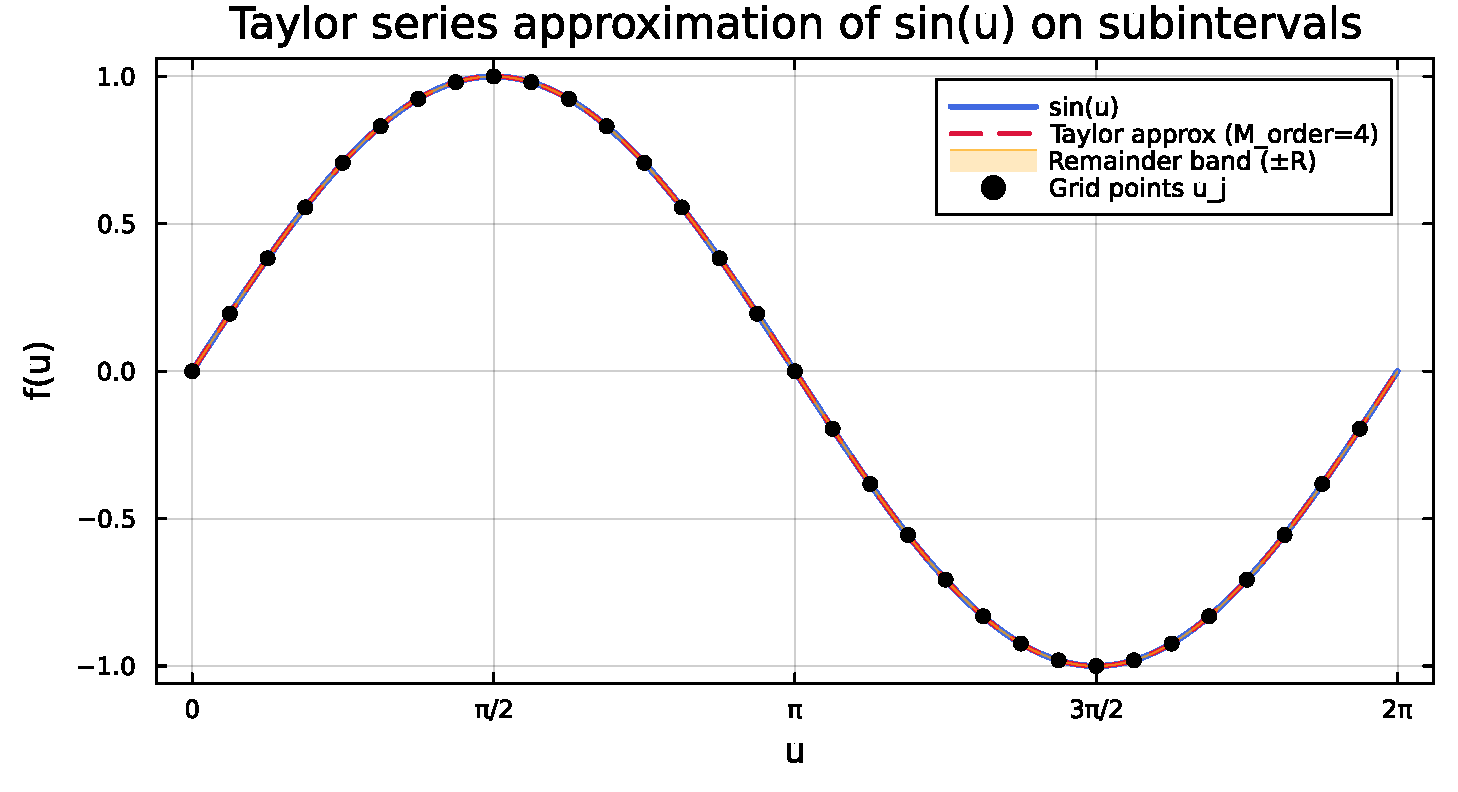
\includegraphics[width=\linewidth]{figures/fig_m2_1.pdf}
  \caption{T2.1: $\sin(u)$ (blue), Taylor approximation from nearest grid point
           (red dashed), and remainder band $\pm R$ (orange shading).
           The shaded band always contains the true curve.
           Grid points $u_j$ (black dots) mark the expansion origins.}
  \label{fig:m3_1}
\end{figure}

\subsection{Test T2.2: \texttt{sup\_bound} exceeds the true maximum}

For $M_{\mathrm{order}} = 2, 4, 6$:
\[
  \texttt{sup\_bound}(\texttt{ts\_sin}) \ge 1.0 = \|\sin\|_\infty.
\]

\textbf{Result: 6/6 assertions pass} (3 orders $\times$ 2 checks each).
All bounds are $\ge 1$ and $< 10$.

\subsection{Test T2.3: Certified \texorpdfstring{$D_{\mathrm{lower}}$}{D\_lower} for \texorpdfstring{$y = 0.1\cos u$}{y=0.1cos(u)}}

For $y(u) = 0.1\cos u$ with $M_{\mathrm{grid}} = 256$, $M_{\mathrm{order}} = 4$:
\begin{align*}
  y_u(u) &= -0.1\sin u, \quad \hat H[y_u](u) = 0.1\cos u,\\
  D(u) &= \sqrt{0.01\sin^2 u + (1 + 0.1\cos u)^2}.
\end{align*}
The minimum is attained at $u = \pi$: $D_{\min} = \sqrt{0 + 0.9^2} = 0.9$.

\texttt{dmin\_bound} (now using \texttt{sqrt\_series} with the rigorous
Fa\`a di Bruno sup\_bounds vector) returns $D_{\mathrm{lower}} \approx 0.89993$.
All three checks pass:

\begin{center}
\begin{tabular}{ll}
\toprule
Check & Value \\
\midrule
$D_{\mathrm{lower}} > 0.88$ (conservative) & 0.8999 $>$ 0.88 \checkmark \\
$D_{\mathrm{lower}} < 0.9$ (it is a lower bound) & 0.8999 $<$ 0.9 \checkmark \\
$D_{\mathrm{lower}} > 0$ (positive) & 0.8999 $>$ 0 \checkmark \\
\bottomrule
\end{tabular}
\end{center}

\textbf{Result: 3/3 assertions pass.}
Figure~\ref{fig:m3_3} shows $D_{\mathrm{lower}}$ vs.\ $M_{\mathrm{grid}}$
converging to $D_{\min} = 0.9$ from below.

\begin{figure}[H]
  \centering
  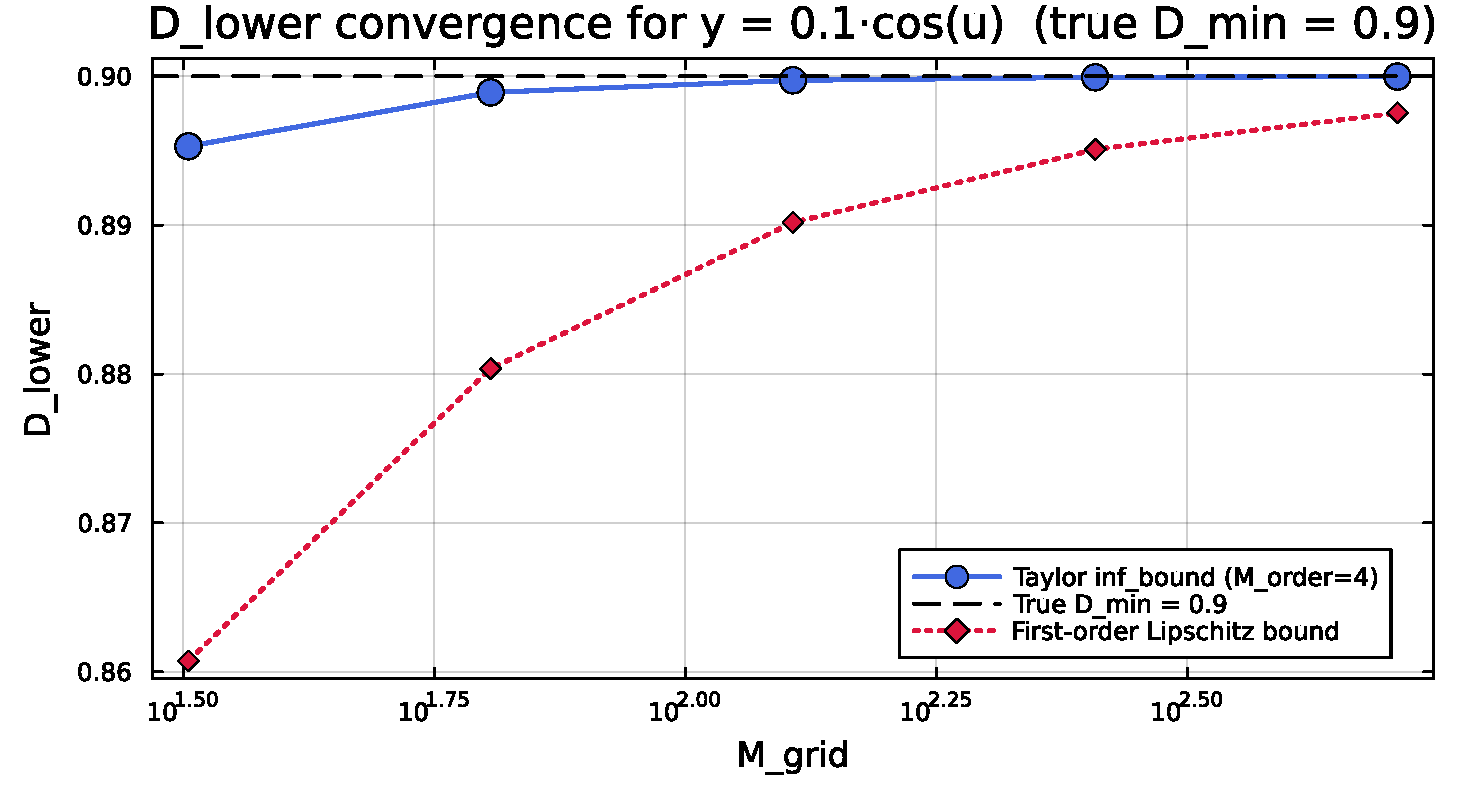
\includegraphics[width=\linewidth]{figures/fig_m2_3.pdf}
  \caption{T2.3: Certified $D_{\mathrm{lower}}$ (blue circles) vs.\ $M_{\mathrm{grid}}$
           for $y = 0.1\cos u$, $M_{\mathrm{order}} = 4$.
           The Taylor bound (blue) converges rapidly to the true $D_{\min} = 0.9$
           (dashed black), while the first-order Lipschitz bound (red dotted)
           is much looser at small $M_{\mathrm{grid}}$.}
  \label{fig:m3_3}
\end{figure}

\subsection{Test T2.4: Remainder decreases with order}

For $M_{\mathrm{grid}} = 32$, we compute $\texttt{sup\_bound}(\texttt{ts\_sin}) - 1$
for $M_{\mathrm{order}} = 1, 2, 3, 4, 5$.
The overestimate (excess above the true $\|\sin\|_\infty = 1$) should decrease
as the Taylor remainder $h^{M+1}/(M+1)!$ decreases.

\textbf{Result: 4/4 assertions pass.}
Figure~\ref{fig:m3_2} shows the overestimate on a log scale; it decays
rapidly with order.

\begin{figure}[H]
  \centering
  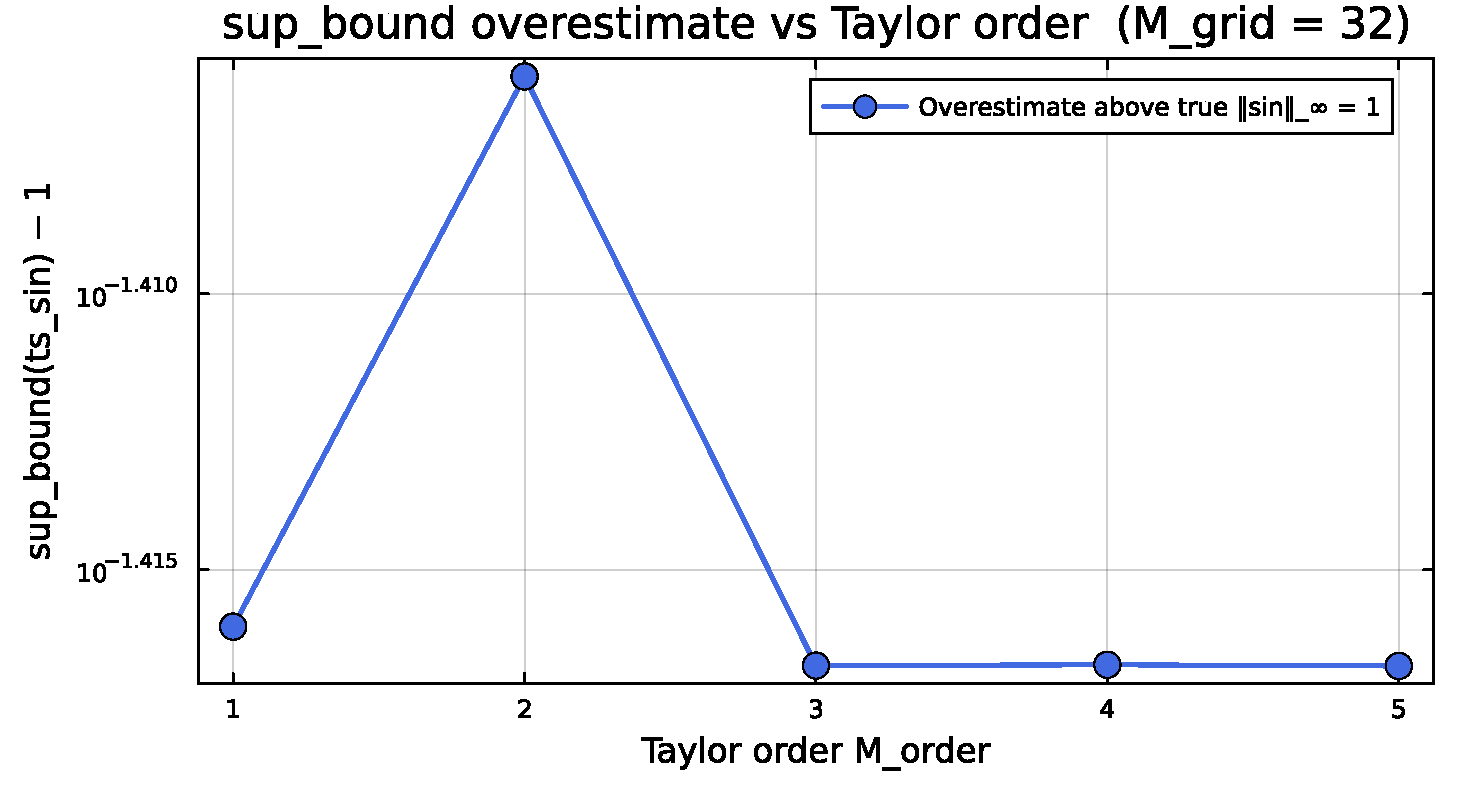
\includegraphics[width=0.75\linewidth]{figures/fig_m2_2.pdf}
  \caption{T2.4: Overestimate $\texttt{sup\_bound}(\texttt{ts\_sin}) - 1$
           vs.\ Taylor order for $M_{\mathrm{grid}} = 32$.
           The bound decreases rapidly, demonstrating that higher Taylor order
           yields tighter certified bounds.}
  \label{fig:m3_2}
\end{figure}

\subsection{Test T2.5: \texttt{deriv\_series}}

\texttt{deriv\_series}(\texttt{ts\_cos}) is checked to agree with
$\texttt{ts}_{-\sin}$ at all 32 grid points for orders $m = 0,\ldots,4$
(since $\cos' = -\sin$).

\textbf{Result: 161/161 assertions pass} (32 points $\times$ 5 orders + 1 order check).
All differences \texttt{contains\_zero} in Arb.

\subsection{Test T2.6: Product}

$\texttt{ts\_sin} \times \texttt{ts\_cos}$ is compared at all grid points and
all derivative orders to the Taylor series for $\sin(u)\cos(u) = \sin(2u)/2$.

\textbf{Result: 160/160 assertions pass} (32 points $\times$ 5 orders).

\subsection{Test T2.7: \texttt{inv\_series}}

For $f(u) = 2 + \cos(u) \ge 1$, \texttt{inv\_series}$(\texttt{ts\_f},\, 1)$
is checked at all 32 grid points: the zeroth-order coefficient equals
$1/(2 + \cos(u_j))$ exactly (both computed by Arb).

\textbf{Result: 34/34 assertions pass} (32 grid checks + 2 range checks).

\subsection{Test T2.8: Product \texttt{sup\_bounds} rigor (audit C4 regression)}

For $f = g = \sin(u)$, we have $f \cdot g = \sin^2(u) = (1 - \cos(2u))/2$
with exact derivative supnorms
\[
  \|(\sin^2)^{(m)}\|_\infty = \begin{cases} 1, & m = 0 \\ 2^{m-1}, & m \ge 1. \end{cases}
\]
The exact-Leibniz formula \eqref{eq:product_fbound} gives, for $\|\sin^{(k)}\|_\infty = 1$ at all $k$,
$\sum_k \binom{m}{k} \cdot 1 \cdot 1 = 2^m$, which is at most $2\times$ the truth
for $m \ge 1$ and tight at $m = 0$. The test verifies
$\texttt{sup\_bounds}_{f g}[m{+}1] \ge \|(\sin^2)^{(m)}\|_\infty$ for every
$m = 0,\ldots,M_{\mathrm{order}}+1$ and every $M_{\mathrm{order}} \in \{2, 4, 6\}$.

\textbf{Result: 18/18 assertions pass.}

\subsection{Test T2.9: \texttt{inv\_series} \texttt{sup\_bounds} responds to input frequency
            (audit C1 regression)}

For $f(u) = 2 + \cos(Nu)$ with $\|f^{(k)}\|_\infty = N^k$ ($k \ge 1$),
the Fa\`a di Bruno bound on $\|(1/f)^{(M+1)}\|_\infty$ should scale roughly
as $N^{M+1}$. At $M_{\mathrm{order}} = 2$, the test records:
\[
  N = 1: \texttt{sup\_bounds}[\mathrm{end}] = 13.0,
  \quad N = 3: 351.0,
  \quad N = 10: 13\,000.
\]
The growth $13 \to 13\,000$ for $N = 1 \to 10$ matches the expected
$N^3 = 1000\times$ scaling (Fa\`a di Bruno single-block term $\phi^{(1)}(f)\cdot f^{(M+1)}$).
The previous formula returned a constant $\approx 162$ independent of $N$ —
unsound by orders of magnitude.

\textbf{Result: 3/3 assertions pass.}

\subsection{Test T2.10: \texttt{sqrt\_series} \texttt{sup\_bounds} responds to input frequency
            (audit C2 regression)}

Same setup as T2.9 but for \texttt{sqrt\_series}. Recorded values:
\[
  N = 1: \texttt{sup\_bounds}[\mathrm{end}] = 1.625,
  \quad N = 3: 43.875,
  \quad N = 10: 1\,625.
\]
The previous formula was dimensionally inconsistent and ignored $f$'s
derivative bounds entirely; the new sup\_bounds vector correctly grows with $N$.

\textbf{Result: 3/3 assertions pass.}

%% -------------------------------------------------------------------
\section{Summary}

\begin{table}[H]
\centering
\begin{tabular}{llcc}
\toprule
Test & Description & Assertions & Result \\
\midrule
T2.1  & Taylor expansion contains true $\sin(u)$ at 200 points & 1 & \textcolor{green!60!black}{\textbf{pass}} \\
T2.2  & \texttt{sup\_bound} $\ge \|\sin\|_\infty = 1$ for orders 2,4,6 & 6 & \textcolor{green!60!black}{\textbf{pass}} \\
T2.3  & $D_{\mathrm{lower}} > 0.88$ for $y = 0.1\cos u$ (true $D_{\min} = 0.9$) & 3 & \textcolor{green!60!black}{\textbf{pass}} \\
T2.4  & \texttt{sup\_bound} decreases with $M_{\mathrm{order}}$ & 4 & \textcolor{green!60!black}{\textbf{pass}} \\
T2.5  & \texttt{deriv\_series}$(\cos) = -\sin$ at all grid points & 161 & \textcolor{green!60!black}{\textbf{pass}} \\
T2.6  & $\texttt{ts\_sin} \times \texttt{ts\_cos} = \texttt{ts}_{\sin(2u)/2}$ & 160 & \textcolor{green!60!black}{\textbf{pass}} \\
T2.7  & \texttt{inv\_series}: $1/(2 + \cos u)$ at 32 grid points & 34 & \textcolor{green!60!black}{\textbf{pass}} \\
T2.8  & Product \texttt{sup\_bounds} $\ge \|(\sin^2)^{(m)}\|_\infty$ (audit C4) & 18 & \textcolor{green!60!black}{\textbf{pass}} \\
T2.9  & \texttt{inv\_series} \texttt{sup\_bounds} scales with $N$ (audit C1) & 3 & \textcolor{green!60!black}{\textbf{pass}} \\
T2.10 & \texttt{sqrt\_series} \texttt{sup\_bounds} scales with $N$ (audit C2) & 3 & \textcolor{green!60!black}{\textbf{pass}} \\
T2.11 & \texttt{\_faa\_di\_bruno\_derivs} against analytic compositions
        $(g\circ C)$ with $g \in \{x,\,x^2,\,\exp\}$, $C \in \{z+1,\,z,\,z^2+z\}$;
        the last verifies derivs $[1,1,3,7]$ at $z=0$ & 12 & \textcolor{green!60!black}{\textbf{pass}} \\
T2.12 & \texttt{dmin\_bound} throws on degenerate $y$ ($D \not> 0$) & 1 & \textcolor{green!60!black}{\textbf{pass}} \\
T2.13 & $M_{\mathrm{order}} = 0$ edge case (smallest legal):
        \texttt{sup\_bound}, $*$, \texttt{deriv\_series} reject, \texttt{inv\_series} & 9 & \textcolor{green!60!black}{\textbf{pass}} \\
T2.14 & \texttt{trigpoly\_to\_taylor}: derivs + sup\_bounds vs.\ analytic $\sin$
        at 32 grid points $\times$ 5 derivative levels & 166 & \textcolor{green!60!black}{\textbf{pass}} \\
\midrule
\textbf{Total} & & \textbf{581} & \textcolor{green!60!black}{\textbf{581/581}} \\
\bottomrule
\end{tabular}
\caption{M2 test summary. All 581 assertions pass at 128-bit Arb precision.
Tests T2.8--T2.10 guard against the audit findings on the old single-scalar
\texttt{F\_bound} formulas. T2.11--T2.14 (post-implementation re-audit) add
direct coverage of \texttt{\_faa\_di\_bruno\_derivs}, the \texttt{dmin\_bound}
throw path, the $M_{\mathrm{order}} = 0$ edge case, and \texttt{trigpoly\_to\_taylor}.}
\end{table}

Milestone M2 is complete. The \texttt{TaylorSeries.jl} module provides:
\begin{itemize}
  \item A certified Taylor-series representation of smooth functions at grid
        points, with a \emph{vector} of supnorm bounds covering every derivative
        order from $0$ to $M_{\mathrm{order}}+1$.
  \item Rigorous \texttt{sup\_bound} and \texttt{inf\_bound} using the remainder
        formula~\eqref{eq:taylor}.
  \item Arithmetic (add, multiply, scale, differentiate) with certified
        \texttt{sup\_bounds} propagation via \emph{exact} Leibniz term-by-term.
  \item Recursive \texttt{inv\_series} and \texttt{sqrt\_series} with
        \texttt{sup\_bounds} via Fa\`a di Bruno (\texttt{ArbSeries} composition).
  \item \texttt{dmin\_bound}$(y)$: a certified lower bound on
        $D = \sqrt{y_u^2 + (1 + \hat H[y_u])^2}$ using only exact
        \texttt{TrigPoly} derivatives (from M1) and the Taylor remainder
        formula.
\end{itemize}

The next milestone will use \texttt{TaylorSeries} to bound all terms in the
Babenko residual operator between grid points, completing the certified
$\|R\|_\infty \le \varepsilon$ estimate.

\end{document}
